%%%%%%%%%%%%%%%%%%%%%%%%%%%%%%%%%%%%%%%%%%%%%%%%%%%%%%%%%%%%%%%%%%%%%%%%%%%%%%%
%     STYLE POUR LES RAPPORTS DE PROJET
%                   NE PAS MODIFIER
%%%%%%%%%%%%%%%%%%%%%%%%%%%%%%%%%%%%%%%%%%%%%%%%%%%%%%%%%%%%%%%%%%%%%%%%%%%%%%%

\documentclass[a4paper,11pt]{article}
\usepackage[utf8]{inputenc}
\usepackage{graphicx}
\usepackage[T1]{fontenc}
\usepackage[latin1]{inputenc}
\usepackage[french]{babel}
\usepackage{float}
\usepackage{wrapfig}
\usepackage{lmodern}
\usepackage{fancyhdr}
\usepackage[top=2cm, bottom=2.7cm,right=1.5cm]{geometry}
\usepackage{tabularx}
\usepackage{array}
\usepackage{longtable}
\usepackage{hyperref}
\usepackage[final]{pdfpages} 
%%%%%%%%%%%%%%%%%%%%%%%%%%%%%%%%%%%%%%%%%%%%%%%%%%%%%%%%%%%%%%%%%%%%%%%%%%%%%%%
\usepackage{listings}
\lstset{language=xml,frame=single, breaklines=true, basicstyle=\ttfamily,backgroundcolor=\color{white},basicstyle=\scriptsize, keywordstyle=\color{blue}, commentstyle=\color{vert}, stringstyle=\color{red}, identifierstyle=\color{blue}}
\lstset{
language=Java,
basicstyle=\normalsize, % ou ça==> basicstyle=\scriptsize,
upquote=true,
aboveskip={1.5\baselineskip},
columns=fullflexible,
showstringspaces=false,
extendedchars=true,
breaklines=true,
showtabs=false,
showspaces=false,
showstringspaces=false,
identifierstyle=\ttfamily,
keywordstyle=\color[rgb]{0,0,1},
commentstyle=\color[rgb]{0.133,0.545,0.133},
stringstyle=\color[rgb]{0.627,0.126,0.941},
}

\makeatletter
\def\clap#1{\hbox to 0pt{\hss #1\hss}}%
\def\ligne#1{%
\hbox to \hsize{%
\vbox{\centering #1}}}%
\def\haut#1#2#3{%
\hbox to \hsize{%
\rlap{\vtop{\raggedright #1}}%
\hss
\clap{\vtop{\centering #2}}%
\hss
\llap{\vtop{\raggedleft #3}}}}%
\def\bas#1#2#3{%
\hbox to \hsize{%
\rlap{\vbox{\raggedright #1}}%
\hss
\clap{\vbox{\centering #2}}%
\hss
\llap{\vbox{\raggedleft #3}}}}%
\def\maketitle{%
\thispagestyle{empty}\vbox to \vsize{%
\haut{}{\@blurb}{}
\vfill
\vspace{1cm}
\par
\hrule height 4pt
\par
\begin{flushleft}
\usefont{OT1}{ptm}{m}{n}
\huge \@title
\end{flushleft}
\par
\hrule height 4pt
\par
\begin{flushright}
\usefont{OT1}{phv}{m}{n}
\Large \@author
\par
\end{flushright}

\vspace{1cm}
\vfill
\vfill
\bas{}{\@location le \@date}{}
}%
\cleardoublepage
}
\def\date#1{\def\@date{#1}}
\def\author#1{\def\@author{#1}}
\def\title#1{\def\@title{#1}}
\def\location#1{\def\@location{#1}}
\def\blurb#1{\def\@blurb{#1}}
\date{\today}
\author{}
\title{}
\makeatother
\title { \textbf{Projet Génie Logiciel - Version 1}\\
Mini-éditeur de texte} 
\author{
        Adeline \textsc{GRANET},\\
        Alexis \textsc{LINARD} \\
 }

\blurb{%
Université de Nantes\\
Master 1 ATAL \\[1em]
} 
%%%%%%%%%%%%%%%%%%%%%%%%%%%%%%%%%%%%%%%%%%%%%%%%%%%%%%%%%%%%%%%%%%%%%%%%%%%%%%%

\begin{document}          


\pagestyle{fancy}
\renewcommand{\headrulewidth}{1pt}
\renewcommand{\footrulewidth}{0pt}
\renewcommand{\headsep}{50pt}
\lhead{Mini-éditeur de texte}
\cfoot{}
\rfoot{\thepage}



\maketitle                 % Genere le titre
\thispagestyle{empty}      % Supprime le numero de page sur la 1re page

\newpage
\tableofcontents

\newpage

\section{Introduction}
\paragraph{}
Le projet \textit{Mini Editeur} a pour but la réalisation d'un outil d'éditeur de texte. Il s'inscrit dans le module de Génie Loiciel. A travers lui, nous apprenons à utiliser différents outils tel que le langage Scala avec sa bibliothèque graphique Swing dans l'IDE\footnote{Integrated Development Environment : ensemble d'outils pour augmenter la productivité des programmeurs qui développent des logiciels} Éclipse ce qui nous permet de compiler, déboguer et utiliser githup pour la gestion de version. 
\paragraph{}
L’objectif de ce rapport est de présenter la modélisation de notre mini-éditeur de texte tel que nous l'avons conçu tout en intégrant les principaux diagrammes d’UML,  certains patrons de conception et ainsi que les techniques liés à l'environnement de travail.
Dans une première partie, nous présenterons le projet. L'éditeur sera présenté de manière approfondi avec ses fonctionnalités.
\paragraph{}
Dans une seconde partie, nous exposerons la vision du projet sous forme de diagramme de classe avec l'explication des patrons de conceptions utilisés. 



\section{Présentation du projet : le Mini-Editeur}
Nous allons présenter dans cette partie l'éditeur de texte dans sa globalité avec les différentes fonctionnalités que l'on devra intégrer ainsi que le contenu de chaque version.

\subsection{Le principe}
Ce projet reste un éditeur de texte tout ce qu'il y a de plus basique avec les fonctionnalités qu'on lui connait. Certains conceptions et fonctionnalités nous ont été imposé comme suit : 
\begin{itemize}
\item le texte est contenu dans un Buffer (zone de travail);
\item il existe une notion de sélection de texte, avec des commandes utilisateur permettant de déplacer le début et la fin de la sélection; 
\item copie de la sélection dans le presse-papier; 
\item copie de la sélection dans le presse-papier puis effacement de la sélection;
\item remplacement de la sélection par le contenu du presse-papier;
\item l'interface homme-machine est d'un type quelconque (textuelle ou graphique).
\end{itemize}
Pour ce dernier point, nous avons choisi une version graphique simple pour interagir avec l'utilisateur.

\subsection{En plusieurs versions}
La conception du logiciel doit se faire en spirale c'est-à-dire fournir des livrables à intervalle donné et enrichir la version précédente à chaque fois. Nous aurons trois version de l'éditeur de texte. 
\begin{description}
\item la version 1 contiendra uniquement les actions d'édition de base ainsi que l'interface graphique correspondante;
\item la version 2 permettra d'enregistrer les actions de l'utilisateur et de les rejouer;
\item la version 3 permettra de réaliser le défaire/refaire, avec une capacité quelconque dans le défaire (c'est-à-dire être capable de revenir à l'état initial)
\end{description}
A chaque étape, nous ferons évoluer l'interface graphique en conséquence de l'ajout/modification des différentes options.

\paragraph{}
Ce projet est conçu pour que l'on puisse répondre à certains objectifs pédagogique qui ont été fixé comme être capable de présenter une tehnique de conception en utilisant différents patrons de conception; être capable de faire en parallèle la réalisation de diagramme statique et dynamique en UML.

\paragraph{}
Dans ce rapport c'est donc la première version que nous allons présenter avec le(s) patron(s) mis en jeu.



\section{Implémentation de la version 1}
\subsection{Patrons de conceptions}

\paragraph{Singleton}
Le but de ce patron de conception est de limiter une classe à une seule et unique instance. 
Pour notre projet, nous avons choisi de mettre la classe \textit{Buffer} en singleton car plusieurs interfaces hommmes-machines peuvent être reliés à un même Buffer mais l'inverse n'est pas possible.

\pargraph{}
Nous avons donc mis le constructeur de la classe en privé aisni que l'instance de la classe, et une méthode publique qui permet de récupérer cette même instance. Sur la figure \ref{Singleton}, on peut voir au bas de la classe, les deux méthodes citées.


\begin{figure}[!ht]
		\center
		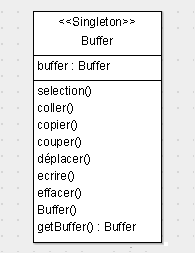
\includegraphics [width=3cm]{singleton.png}
		\caption{Mise en oeuvre du patron Singleton}
		\label{singleton}
\end{figure}

\paragraph{Commande} Ce patron de conception est de type comportemental. Ce patron va permettre d'encapsuler une action réalisée par l'utilisateur (autrement appellée requête)  dans un objet pour permettre diverses opérations sur la requête. Cela va permettre de dissocier l'objet qui invoque une opération de l'objet qui possède les connaissances nécessaires pour réaliser l'opération demandée. On peut voir l'invocateur comme l'instrument qui appelle la méthode à exécuter. Il est particulièrement recommandé en présence d'une IHM car il permet une certaine flexibilité au niveau du design comme le partage de fonctionnalités et le remplacement dynamique des commandes.
\paragraph{}
Concrètement, nous avons appliqué le patron sur notre projet comme suit : \\

\begin{table}[H]
\caption{Distribution des rôles}
\center
\begin{tabular}{||l|c||}
\hline
\textbf{Rôle} & \textbf{Objet}\\
\hline\hline
Client & IHM \\
\hline
Invocateur & IHM \\
\hline
Commande & Command \\
\hline
CommandeConcrète & Cut, Paste, Copy, Move,  Select \\
\hline
Receveur & Buffer \\
\hline
\end{tabular}
\end{table}

\paragraph{}
Maintenant que nous avons explicité le rôle de chacun ainsi que les interactions qu'il existe entre eux, nous vous présentons en figure \ref{command} le diagramme de classe correspondant à notre projet et mettant en œuvre le patron Commande.

\begin{figure}[!ht]
		\center
		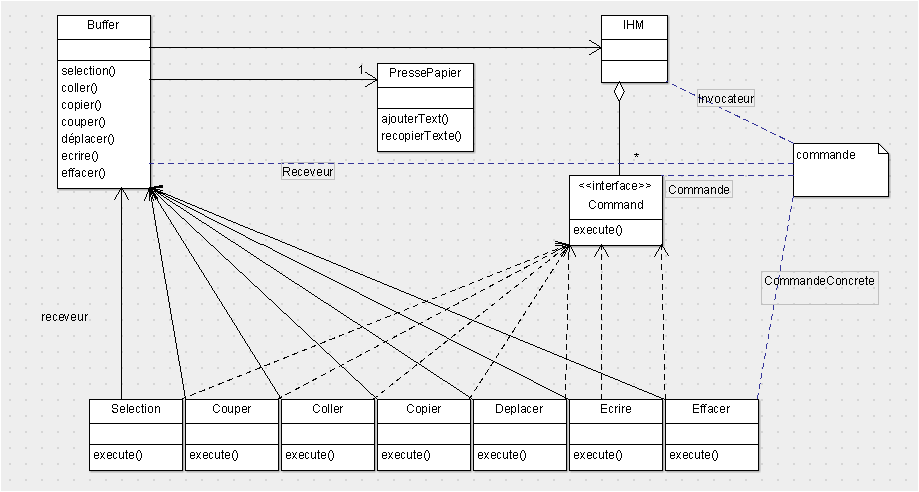
\includegraphics [width=15cm]{Command.png}
		\caption{Mise en oeuvre du patron Commande}
		\label{command}
\end{figure}

\paragraph{}
Afin d'expliciter un peu plus encore le fonctionnement, nous présentons en figure \ref{seq1} et \ref{seq2} des exemples de diagramme de séquence où l'on peut voir les interactions entre chaque classe.

\begin{figure}[!ht]
		\center
		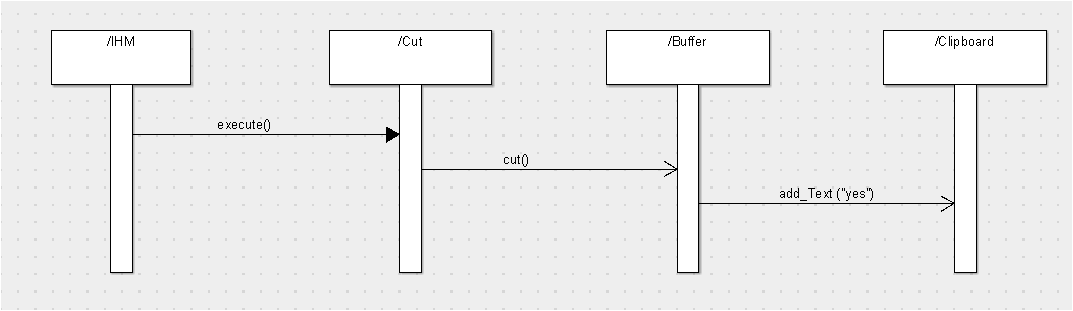
\includegraphics [width=15cm]{seq1.png}
		\caption{Diagramme de séquence pour couper}
		\label{seq1}
\end{figure}

\begin{figure}[!ht]
		\center
		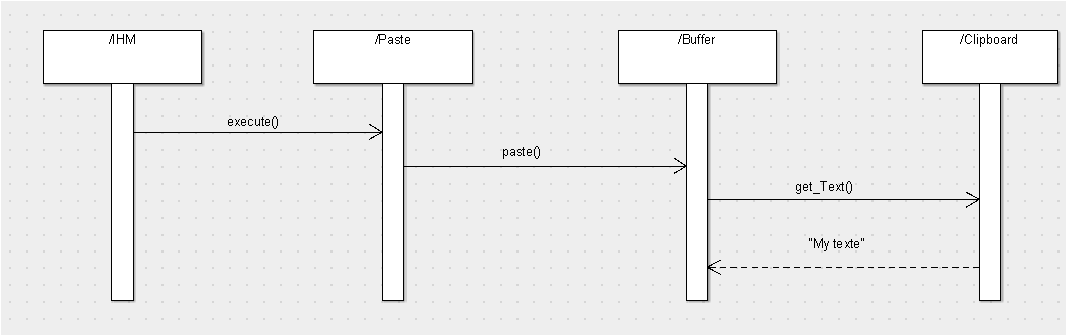
\includegraphics [width=15cm]{seq2.png}
		\caption{Diagramme de séquence pour coller}
		\label{seq2}
\end{figure}

\begin{figure}[!ht]
		\center
		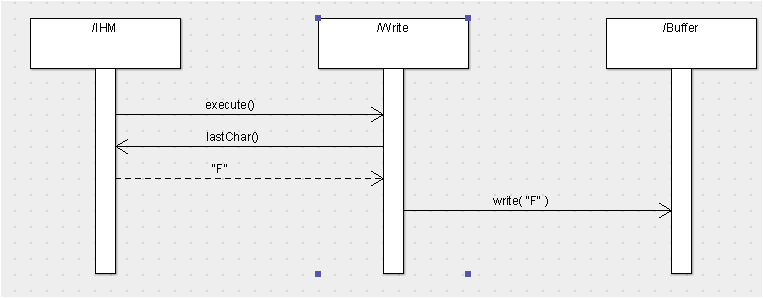
\includegraphics [width=15cm]{seq3.png}
		\caption{Diagramme de séquence pour écrire}
		\label{seq3}
\end{figure}

\subsection{Interface graphique}
Nous présentons en figure \ref{ui}, l'interface que nous avons réalisé pour l'utilisateur. 
D'un point de vue générale, nous avons deux parties distinctes dans cette interface : la partie éditeur avec l'espace pour écrire du texte et la partie interaction avec les boutons. On y retrouve les différentes fonctions qui nous ont été demandé : copier, coller, couper. 
Il y a également deux autres boutons qui sont désactivés pour l'instant car ils sont en préparation pour la prochaine version avec le concept \textit{undo/redo}. Grâce à Scala et à la classe \texttt{TextArea}, nous n'avons pas eu besoin de créer un bouton \textit{select} car la sélection de texte se fait avec la souris.
\begin{figure}[!ht]
		\center
		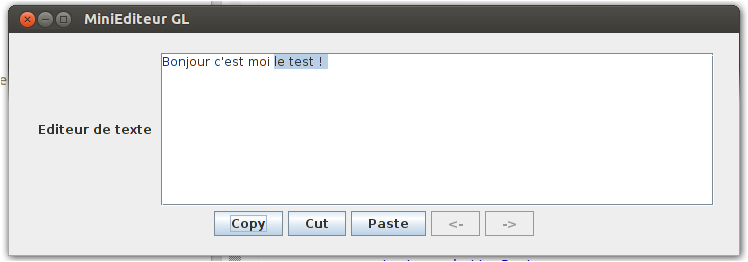
\includegraphics [width=10cm]{ui.png}
		\caption{L'interface graphique réalisée}
		\label{ui}
\end{figure}


\newpage
\section{Conception Détaillé}

Dans ce paragraphe, nous décrivons les technologies employées et les moyens utilisés pour implémenter la modélisation décrite précédement.
 
\subsection{Scala}

Scala est un langage de programmation multi-paradigme pour exprimer les modèles de programmation courants dans une forme concise et élégante.

Scala intègre les paradigmes de programmation orientée objet et de programmation fonctionnelle, avec un typage statique. Il concilie ainsi ces deux paradigmes habituellement opposés et offre au développeur la possibilité de choisir le paradigme le plus approprié à son problème. C'est pour cela qu'en tant que développeurs, nous avons l'impression de développer à la fois en Java, et en OCamL !

Ce langage est prévu pour être compilé en bytecode Java (exécutable sur la JVM)

	\begin{figure}[!ht]
		\center
		
\includegraphics [width=50mm]{scala.png}
		\caption{Scala}
	\end{figure}
	
\newpage
\subsubsection{Exemple d'implémentation : le pattern Singleton}

\begin{lstlisting}[caption=Exemple de scaladoc, label=java]

/**
 * Singleton Container
 */
object Buffer {

   val singleton = new Buffer

   def getInstance: Buffer = {
      return singleton;
   }

}

/**
 *
 * Class containing the Buffer
 * @author AdelineAlex
 *
 */
class Buffer {

	val clipBoard = new Clipboard

	val texte = new StringBuffer
	

	/**
	 * Method to copy a text
	 */
	def copy(t: String): Unit = {
		clipBoard.setText(t)
		println(t+" copied into clipboard")
	}

	...

}

\end{lstlisting}	

\subsection{Maven}
Apache Maven est un outil logiciel libre pour la gestion et l'automatisation de production des projets logiciels Java et Java EE en particulier. L'objectif recherché est comparable au système Make sous Unix, que nous étudions dans le cadre du module \textit{Concepts et Outils de Développement} : produire un logiciel à partir de ses sources, en optimisant les tâches réalisées à cette fin et en garantissant le bon ordre de fabrication. Contrairement à Make et aux Autotools, Maven est plus adapté à Java, et surtout bien plus utilisé dans le monde du travail (Make est pour aisi dire déprécié).

	\begin{figure}[!ht]
		\center
		
\includegraphics [width=50mm]{maven.png}
		\caption{Apache Maven}
	\end{figure}

Maven impose une arborescence et un nommage des fichiers du projet. En voici une liste non exhaustive :
	\begin{itemize}
		\item \texttt{/src} : les sources du projet
		\item \texttt{/src/main} : code source et fichiers source principaux
		\item \texttt{/src/main/scala} : code source
		\item \texttt{/src/main/resources} : fichiers de ressources (images, fichiers annexes etc.)
		\item \texttt{/src/main/webapp} : webapp du projet (lorsque projet web - ce n'est pas notre cas)
		\item \texttt{/src/test} : fichiers de test
		\item \texttt{/src/test/scala} : code source de test
		\item \texttt{/src/test/resources} : fichiers de ressources de test
		\item \texttt{/target} : fichiers résultat, les binaires (du code et des tests), les packages générés et les résultats des tests
	\end{itemize}
	
Maven utilise un paradigme connu sous le nom de Project Object Model (POM) afin de décrire un projet logiciel, ses dépendances avec des modules externes et l'ordre à suivre pour sa production. Il est livré avec un grand nombre de tâches pré-définies, comme :
	\begin{itemize}
		\item \texttt{clean} : permet de supprimer le contenu du répertoire /target
		\item \texttt{compile} : permet la compilation du code source
    	\item \texttt{test} : permet l'exécution des tests unitaires
    	\item \texttt{package} : permet la génération d'une release (génération d'une archive JAR et de la scaladoc)
	\end{itemize}

De plus, l'idée est que, pour n'importe quel but, tous les buts en amont doivent être exécutés sauf s'ils ont déjà été exécutés avec succès et qu'aucun changement n'a été fait dans le projet depuis.


Dans le cadre du projet \textsc{MiniEditeur}, nous utilisons cet outil essentiellement pour la gestion des dépendances, afin d'éviter d'importer les archives .jar dans le classpath "à la main". Voici un extrait du \texttt{pom.xml} pour le projet :
\begin{lstlisting}[caption=Exemple de fichier pom.xml, label=ruleml]
<project xmlns="http://maven.apache.org/POM/4.0.0" xmlns:xsi="http://www.w3.org/2001/XMLSchema-instance"
	xsi:schemaLocation="http://maven.apache.org/POM/4.0.0 http://maven.apache.org/xsd/maven-4.0.0.xsd">
	<modelVersion>4.0.0</modelVersion>
	<groupId>MiniEditeur</groupId>
	<packaging>jar</packaging>
	<artifactId>MiniEditeur</artifactId>
	<version>1.0.0-SNAPSHOT</version>
	<name>MiniEditeur</name>
	<description>MiniEditeur projet Genie Logiciel - Adeline Granet and Alexis Linard</description>
	
		...
	
	<dependencies>
	
		...
	
		<dependency>
			<groupId>org.scala-lang</groupId>
			<artifactId>scala-swing</artifactId>
			<version>2.11.0-M5</version>
		</dependency>
		<dependency>
			<groupId>junit</groupId>
			<artifactId>junit</artifactId>
			<version>4.11</version>
		</dependency>
	</dependencies>
		...
</project>
\end{lstlisting}



\subsection{Ajout et génération de scaladoc}
Scaladoc est un outil permettant de créer une documentation d'API en format HTML depuis les commentaires présents dans un code source en Scala. Scaladoc est le standard industriel pour la documentation des classes Scala. En outre, cela permet de commenter convenablement le code de notre mini éditeur. Les développeurs utilisent certains styles de commentaire et des tags Scaladoc\footnote{sur le modèle de la Javadoc, son homologue dans le cas de programmes codés en Java} quand ils documentent un code source. Un bloc de commentaire scala commençant par /** deviendra un bloc de commentaire Scaladoc qui sera inclus dans la documentation du code source. Les commentaires scaladoc précèdent généralement les déclarations de classes, d'attributs et de méthodes. Voici certains tags (liste non exhaustive), et un exemple mis en pratique dans le projet \textsc{MiniEditeur} :
	\begin{itemize}
		\item \texttt{@author} : Nom du développeur
		\item \texttt{@deprecated} : Marque la méthode comme dépréciée. Certains IDEs créent un avertissement à la compilation si la méthode est appelée.
		\item \texttt{@exception} : Documente une exception lancée par une méthode — voir aussi \texttt{@throws}
		\item \texttt{@param} : Définit un paramètre de méthode. Requis pour chaque paramètre.
		\item \texttt{@return} : Documente la valeur de retour. Ce tag ne devrait pas être employé pour des constructeurs ou des méthodes définis avec un type de retour void.
		\item \texttt{@see} : Documente une association à une autre méthode ou classe.
		\item \texttt{@since} : Précise à quelle version de la SDK/JDK une méthode a été ajoutée à la classe.
		\item \texttt{@throws} : Documente une exception lancée par une méthode.
		\item \texttt{@version} : Donne la version d'une classe ou d'une méthode.
	\end{itemize}

	
\newpage
\begin{lstlisting}[caption=Exemple de scaladoc, label=java]
/**
 *
 * Class containing the User Interface
 * @author AdelineAlex
 * @todo une belle IHM dans une webapp peut être
 *
 */
object UserInterface extends SimpleSwingApplication {

	/**
	 * Variable containing the copied value in the text editor
	 */
	var copiedValue: String = ""
	
	/**
	 * @TODO For Saved Actions
	 */
	var debut: Int = 0

	/**
	 * @TODO For Saved Actions
	 */
	var fin: Int = 0

	/**
	 * The UI
	 */
	def top = new MainFrame {

		//Title of the frame
		title = "MiniEditeur GL"
			...
	}
}

\end{lstlisting}	





\subsection{Création d'un repository GitHub et utilisation de GIT}
Dans le but de permettre le développement collaboratif de notre application, nous avons crée un dépôt GitHub pour l'hébergement du projet. Il repose sur \textit{GIT}, qui est un logiciel de gestion de versions. L'avantage de ce procédé est de garder une trace des développements, et de savoir qui a fait quoi, et dans une moindre mesure de réprimander le développeur ayant introduit une régression !

Voici le lien pour le projet :
\begin{center}
\url{https://github.com/allinard/miniEditeurGL}
\end{center}

Les commandes GIT que nous avons le plus utilisé pour le moment sont les suivantes :
\begin{itemize}
		\item \texttt{git init} crée un nouveau dépôt.
		\item \texttt{git clone} clone un dépôt distant.
		\item \texttt{git add} ajoute de nouveaux fichiers au repository.
		\item \texttt{git commit} valider des changements dans un fichier. N'envoie pas sur le repository distant.
		\item \texttt{git branch} crée une nouvelle branche de développement.
		\item \texttt{git merge} fusionne plusieurs branches de développement.
		\item \texttt{git pull} récupérer la version la plus à jour du projet depuis le repository distant.
		\item \texttt{git push} envoyer ses changements sur le repository distant.
\end{itemize}



\subsection{Virtualisation du projet}

Dans un souci d'efficience maximum, nous avons décidé de travailler sur des machines virtuelles\footnote{En informatique, une machine virtuelle (anglais virtual machine, abr. VM) est une illusion d'un appareil informatique créée par un logiciel d'émulation. Le logiciel d'émulation simule la présence de ressources matérielles et logicielles telles que la mémoire, le processeur, le disque dur, voire le système d'exploitation et les pilotes, permettant d'exécuter des programmes dans les mêmes conditions que celles de la machine simulée}. L'avantage de cette pratique est la portabilité de la VM d'un hôte à l'autre. Ainsi, une fois le projet correctement configuré (avec un bon IDE Eclipse bien configuré, et les bons plug-in par exemple), il suffit de la copier d'un collaborateur au projet à un autre. C'est ainsi un bon moyen de ne pas perdre de temps, et de configurer le projet une seule fois.

\begin{figure}[!ht]
		\center
		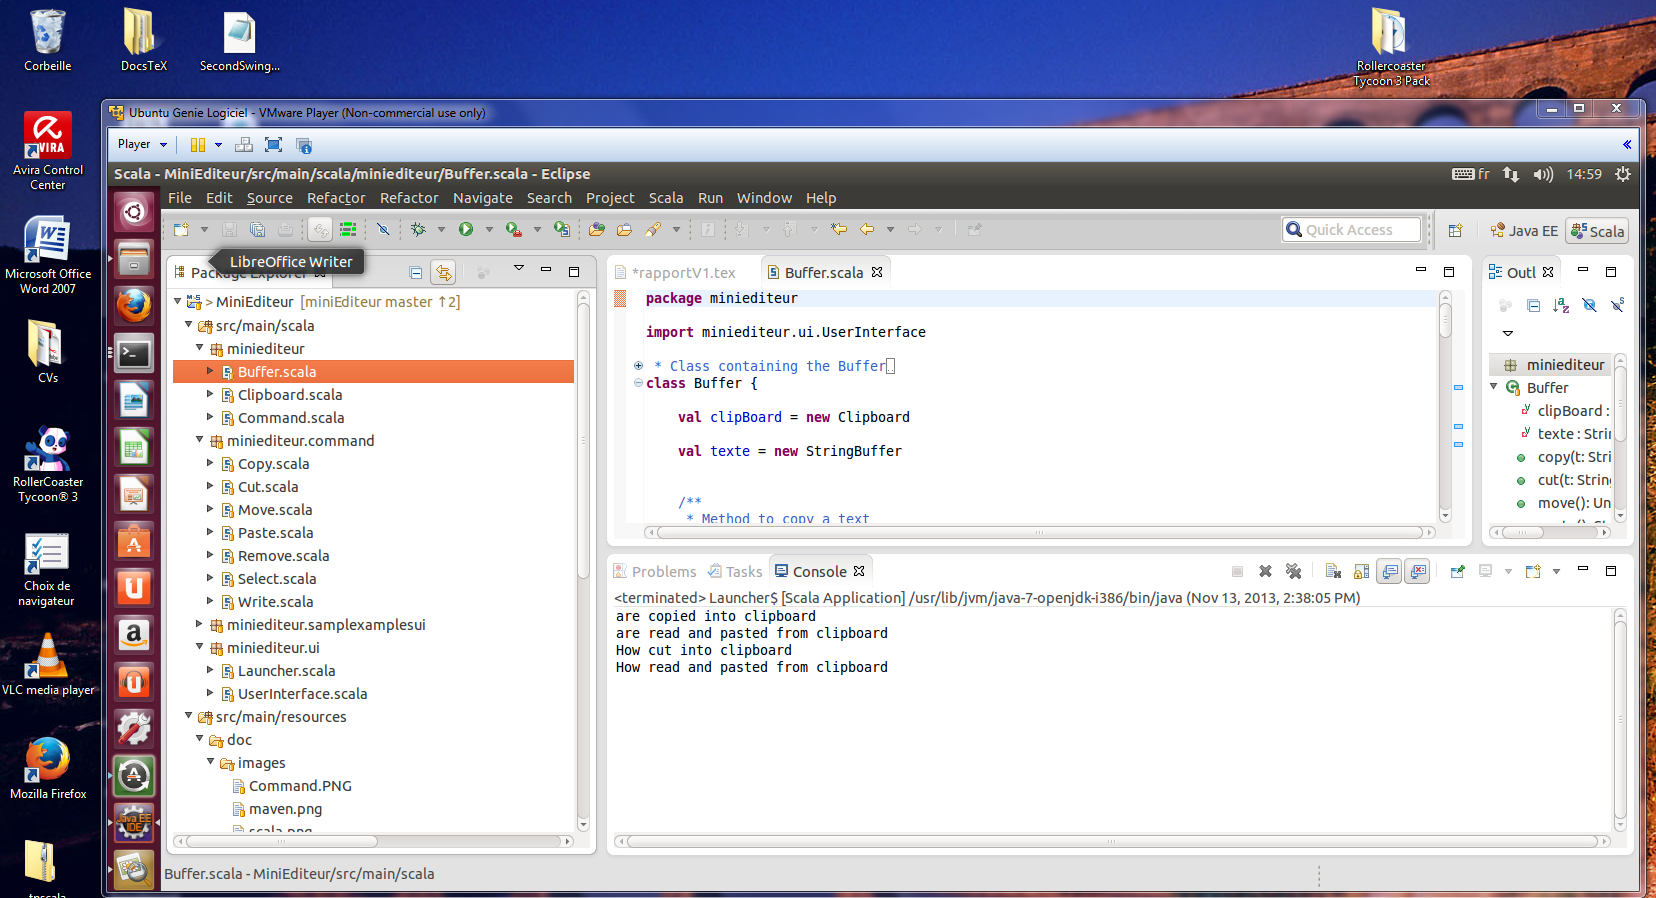
\includegraphics [width=120mm]{vm1.png}
		\caption{Exécution de la VM de développement \textsc{OpenDataWrapper}}
\end{figure}

Cependant, un des inconvénients de l'utilisation des machines virtuelles est le besoin de ressources convenables venant de l'hôte. Dans le cas de notre VM :
\begin{itemize}
\item 3Go RAM (at least)
\item 2 cores
\item + or - 10Go Hard Drive
\end{itemize} 




\section{Tests Unitaires}

Lors du développement d'un logiciel, on peut facilement faire des modifications sans se rendre compte qu'elles introduisent des bugs dans certains cas particuliers : les régressions. Une régression est l'introduction de nouveaux bugs à la suite d'une évolution fonctionnelle. Hors, il n'est pas humainement possible de tester systématiquement tous les cas d'utilisation possible, ces bugs peuvent se retrouver déployés en production, avec tous les problèmes que cela comporte.

Les tests unitaires servent également à cadrer le développement, puisque dans la mesure du possible ils doivent être écrits avant de coder : il s'agit du TDD\footnote{Technique de développement de logiciel qui préconise d'écrire les tests unitaires avant d'écrire le code source d'un logiciel. Ces tests permettent aussi de préciser les spécifications du code et donc son comportement ultérieur en fonction des situations auxquelles il sera exposé. Ce qui facilite la production d'un code valide en toutes circonstances. On obtient donc un code plus juste et plus fiable.}.

Concrètement, les tests unitaires consistent en un ensemble de scripts, qui ont chacun en charge la validation d'un morceau de code (ou d'une classe dans le cadre de la programmation orientée objet). Il existe de très nombreux frameworks : JUnit (Java), SimpleTest (PHP), CppUnit (C++), JSUnit (Javascript), unittest (Python), NUnit (.NET), etc.

Nous avons réalisé nos tests unitaires avec \textsc{JUnit}, qui est décrit ci-dessous. Cependant, nous connaissons également \textsc{ScalaTest}, que nous n'avons pas encore mis en place, ce que nous ferons peut être dans les prochaines versions du mini éditeur...

\subsection{JUnit}

JUnit est un framework de test unitaire initialement développé pour le langage de programmation Java, et qui possède des extensions pour le langage Scala.

JUnit définit deux types de fichiers de tests. Les TestCase sont des classes contenant un certain nombre de méthodes de tests. Un TestCase sert généralement à tester le bon fonctionnement d'une classe. Une TestSuite permet d'exécuter un certain nombre de TestCase déjà définis.

Enfin, JUnit est intégré par défaut dans les environnements de développement intégré Java tels que BlueJ, Eclipse et NetBeans. C'est donc une constante dans le monde de l'entreprise et du développement logiciel !


\subsection{La réalisation concrète de tests unitaires avec Scala}

Voici un exemple simple de test unitaire en Scala :

\newpage
\begin{lstlisting}[caption=Exemple de TU Scala, label=java]
import junit.framework._
import org.junit.Assert._

/**
 * @author AdelineAlexis
 */
class SampleScalaUnitTest extends TestCase {

	/**
	 * Test de la méthode testOne()
	 * @return OK
	 */
	def testOne() = {
		assertEquals(1, 1)
	}

	/**
	 * Test de la méthode testTwo()
	 * @return FAIL
	 */
	def testTwo() = {
		assertEquals(2, 3)
	}

}

\end{lstlisting}	



\newpage
\section{Conclusion}
Cette première modélisation que nous avons réalisé pour l'éditeur de texte est une réponse au cahier des charges qui nous a été fourni. Grâce à cela, nous avons pu définir et mettre en place les principales fonctionnalités que l'éditeur doit posséder. 

\paragraph{}
La réalisation du diagramme de classe, nous a permis de manipuler le patron de conception que l'on a abordé en cours et de le mettre en œuvre. Les diagrammes de séquences nous ont permit de mieux comprendre et analyser comment les différents objets de l'éditeur pouvaient interagir entre eux lors d'une action. 

\paragraph{}
Nous avons également pu réfléchir sur l'agencement de l'interface utilisateur pour qu'elle reste le plus simple possible pour ce dernier tout en restant le plus fonctionnel possible. Tout en sachant que nous devrons l'adapter à chaque version du projet. 

\paragraph{}
La prochaine version devra permettre d'enregistrer les actions de l'utilisateur et de les rejouer. 




\newpage
\listoffigures  % table des figures
\listoftables
\newpage
\nocite{*}
\bibliographystyle{unsrt} % Le style est mis entre accolades.
\bibliography{biblio} % mon fichier de base de données s'appelle bibli.bib
\newpage



\end{document}
